\documentclass[12pt]{article}
\usepackage[english]{babel}
\usepackage[utf8x]{inputenc}
%\usepackage[a4paper, total={6in, 8in}]{geometry}
\usepackage[margin=0.5in]{geometry}
\usepackage{graphicx}
\usepackage{subcaption}
\usepackage{placeins}
\usepackage{hyperref} 
\renewcommand{\thesubsection}{\thesection.\alph{subsection}}

\hypersetup{
    colorlinks=true,
    urlcolor=blue,       % Controls the color of \href and \url links
    linkcolor=black,     % Controls internal links (sections, figures, tables)
    citecolor=green      % Controls bibliography citations
}

%-------------- TITLE -----------------%
\author{James Ogle}
\title{ECE414 -- Final Report}

%---------- START DOCUMENT ------------%
\begin{document}
    \pagenumbering{gobble}
    \maketitle
    \pagenumbering{arabic}
    \begin{center}
        \href{https://github.com/jaogle04/Robot-Search-Algo/tree/master}{Robot Search Algorithm Github Repository}
    \end{center}

    %-----------------------------------------%
    \section*{Project Overview}
    This project develops an autonomous lunar-rover navigation agent that must reach a beacon in a randomly generated $11 \times 11$ grid.
    The rover observes only a local $3 \times 3$ field of view, and obstacles, wall collisions, and a 15\% stochastic movement failure make complete, reliable control difficult.
    The final Deep Q-Network (DQN) learned from partial observations while generalizing across new obstacle layouts; in a 200-episode randomized-grid evaluation it reached the goal in 140 episodes (70\%), compared with 7.5\% for a random policy.
    Although the final rendered test achieved 80\% success, it did not consistently reach the original goal of 80--90\% across all test conditions.
    
    \begin{figure}[ht]
        \centering
        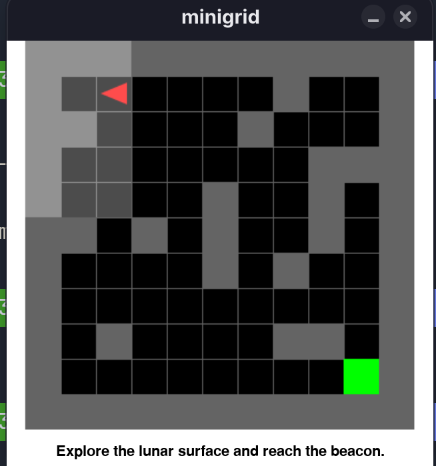
\includegraphics[width=0.55\textwidth]{./img/image_of_grid.png}
        \caption{The lunar-rover environment: the rover starts at $(1,1)$, the beacon is at $(9,9)$, black cells are obstacles, and the gray region is the rover's local partial observation.}
        \label{fig:environment}
    \end{figure}

    \FloatBarrier

    %-----------------------------------------%
    \section*{Final Implementation}
    \textbf{Environment.}
    Grid generation randomly places 16 obstacles, but breadth-first search rejects layouts that do not provide a route from the start to the goal.
    Each episode begins from a new map and ends after reaching the beacon or 150 steps.
    The four actions move east, south, west, or north.
    Rewards are $-0.01$ per step, $-0.05$ for an obstacle collision, $-0.25$ for stochastic movement failure, $+0.02$ for each newly discovered cell, and $+1.0$ for reaching the goal.

    \textbf{Algorithm.}
    The final policy is a DQN with two 128-unit fully connected hidden layers.
    The input combines normalized partial-grid pixels and the rover direction.
    Training uses epsilon-greedy exploration, replay memory, a separately updated target network, the Adam optimizer, and smooth-L1 loss.
    Replay memory reduced correlation between consecutive samples and allowed the network to learn from transition batches collected across many different grids.

    \textbf{Technical challenges and changes.}
    Tabular Q-learning did not generalize to random layouts because its state key effectively encoded local observations encountered during training.
    The DQN was therefore substituted as the final algorithm.
    A replay capacity of 10,000 transitions, batch size of 128, learning rate of $10^{-3}$, discount factor of 0.95, and target-network updates every 100 optimization steps were used for 3,000 training episodes.
    Partial observability and stochastic motion remained difficult: the agent could identify useful behavior in individual episodes while still lacking enough information to consistently recover from unfamiliar layouts.

    \begin{figure}[ht]
        \centering
        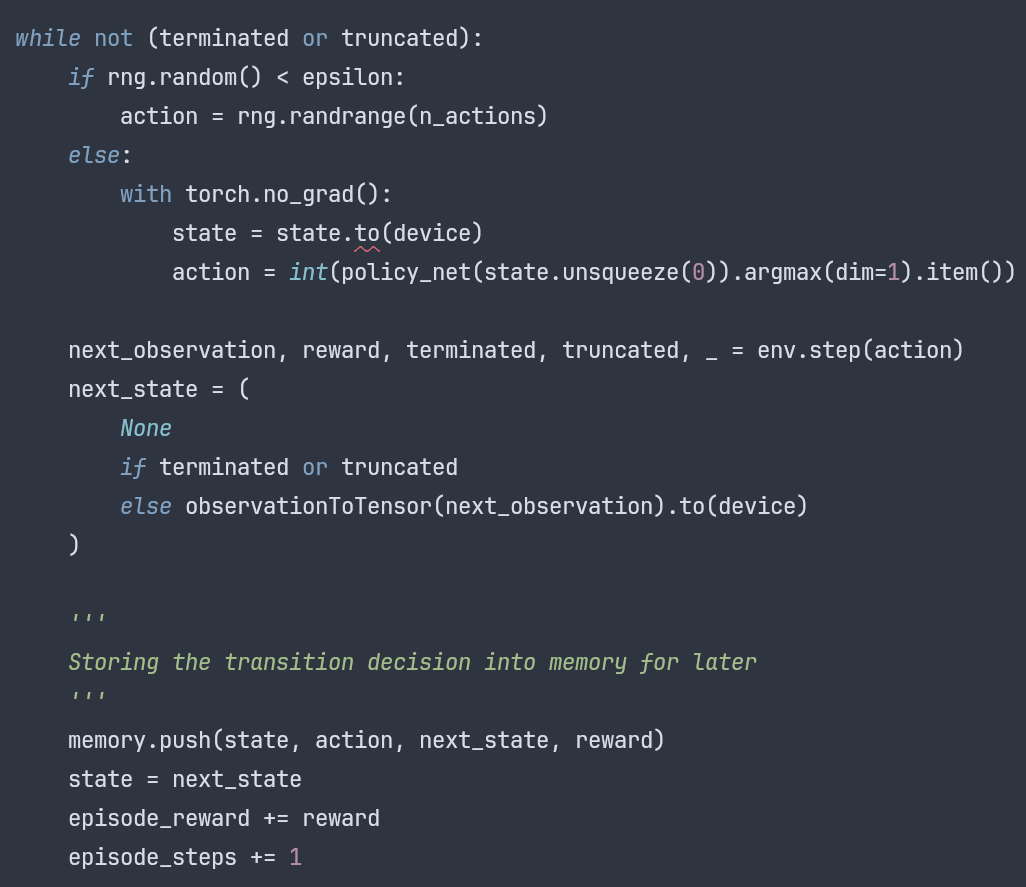
\includegraphics[width=0.55\textwidth]{./img/storing_transitions.png}
        \caption{DQN transition storage and replay-batch optimization used during training.}
        \label{fig:implementation}
    \end{figure}

    %-----------------------------------------%
    \section*{Experimental Setup}
    Performance was measured by episode reward, steps per episode, and whether the rover reached the goal.
    I compared the DQN with tabular Q-learning trained across newly generated grids and with a uniform random-policy baseline.
    The DQN ran for 3,000 training episodes and 200 randomized-grid evaluation episodes.
    Q-learning used learning rate $\alpha=0.1$, discount factor $\gamma=0.95$, epsilon decaying from 1.0 to 0.05, and 2,000 randomized training episodes.
    The final policies were then loaded by separate test scripts and demonstrated on newly generated maps.
    The random policy was evaluated for 1,000 episodes and provides the lowest-complexity baseline.
    A 200-episode DQN evaluation and recorded 5- and 10-episode rendered tests are reported separately because the latter include fewer, stochastic samples.
    
    %-----------------------------------------%
    \section*{Final Results \& Comparisons}
    \begin{figure}[ht]
        \centering
        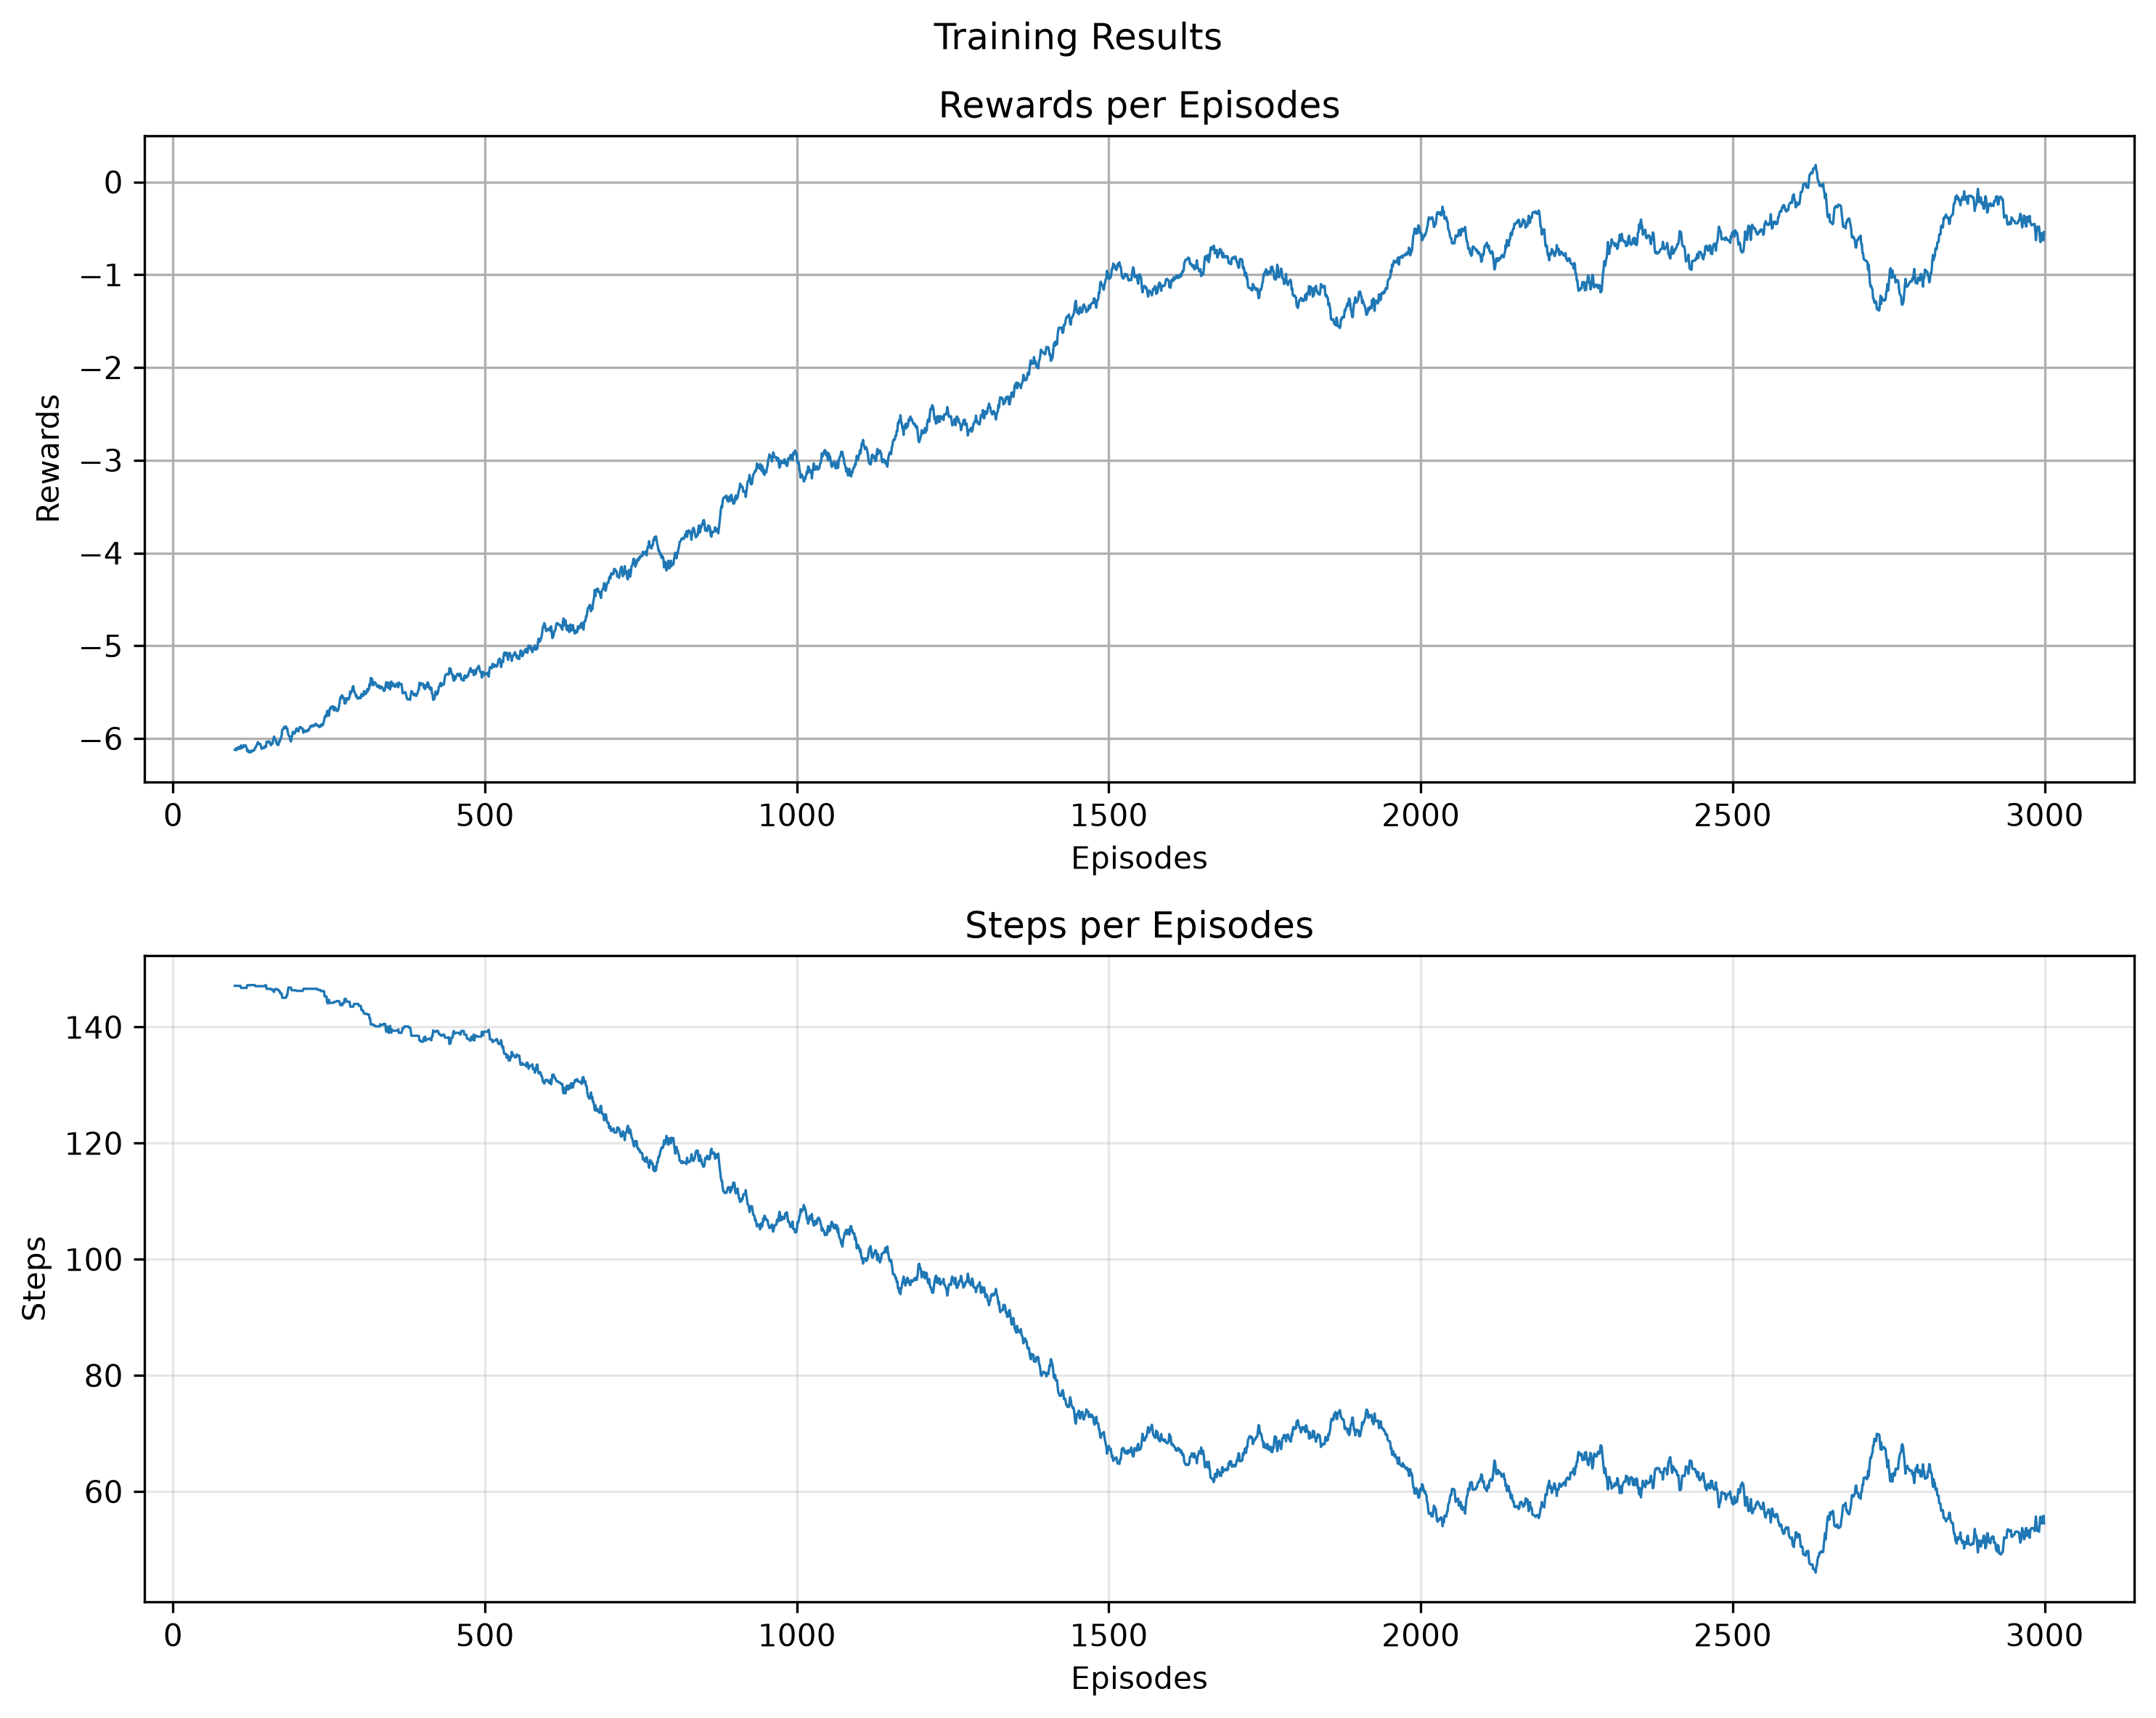
\includegraphics[width=0.72\textwidth]{./img/dqn_train.png}
        \caption{DQN training reward and step curves over 3,000 episodes. The moving-average trend shows improvement before some late-training variability.}
        \label{fig:dqn-training}
    \end{figure}

    \FloatBarrier

    \begin{figure}[ht]
        \centering
        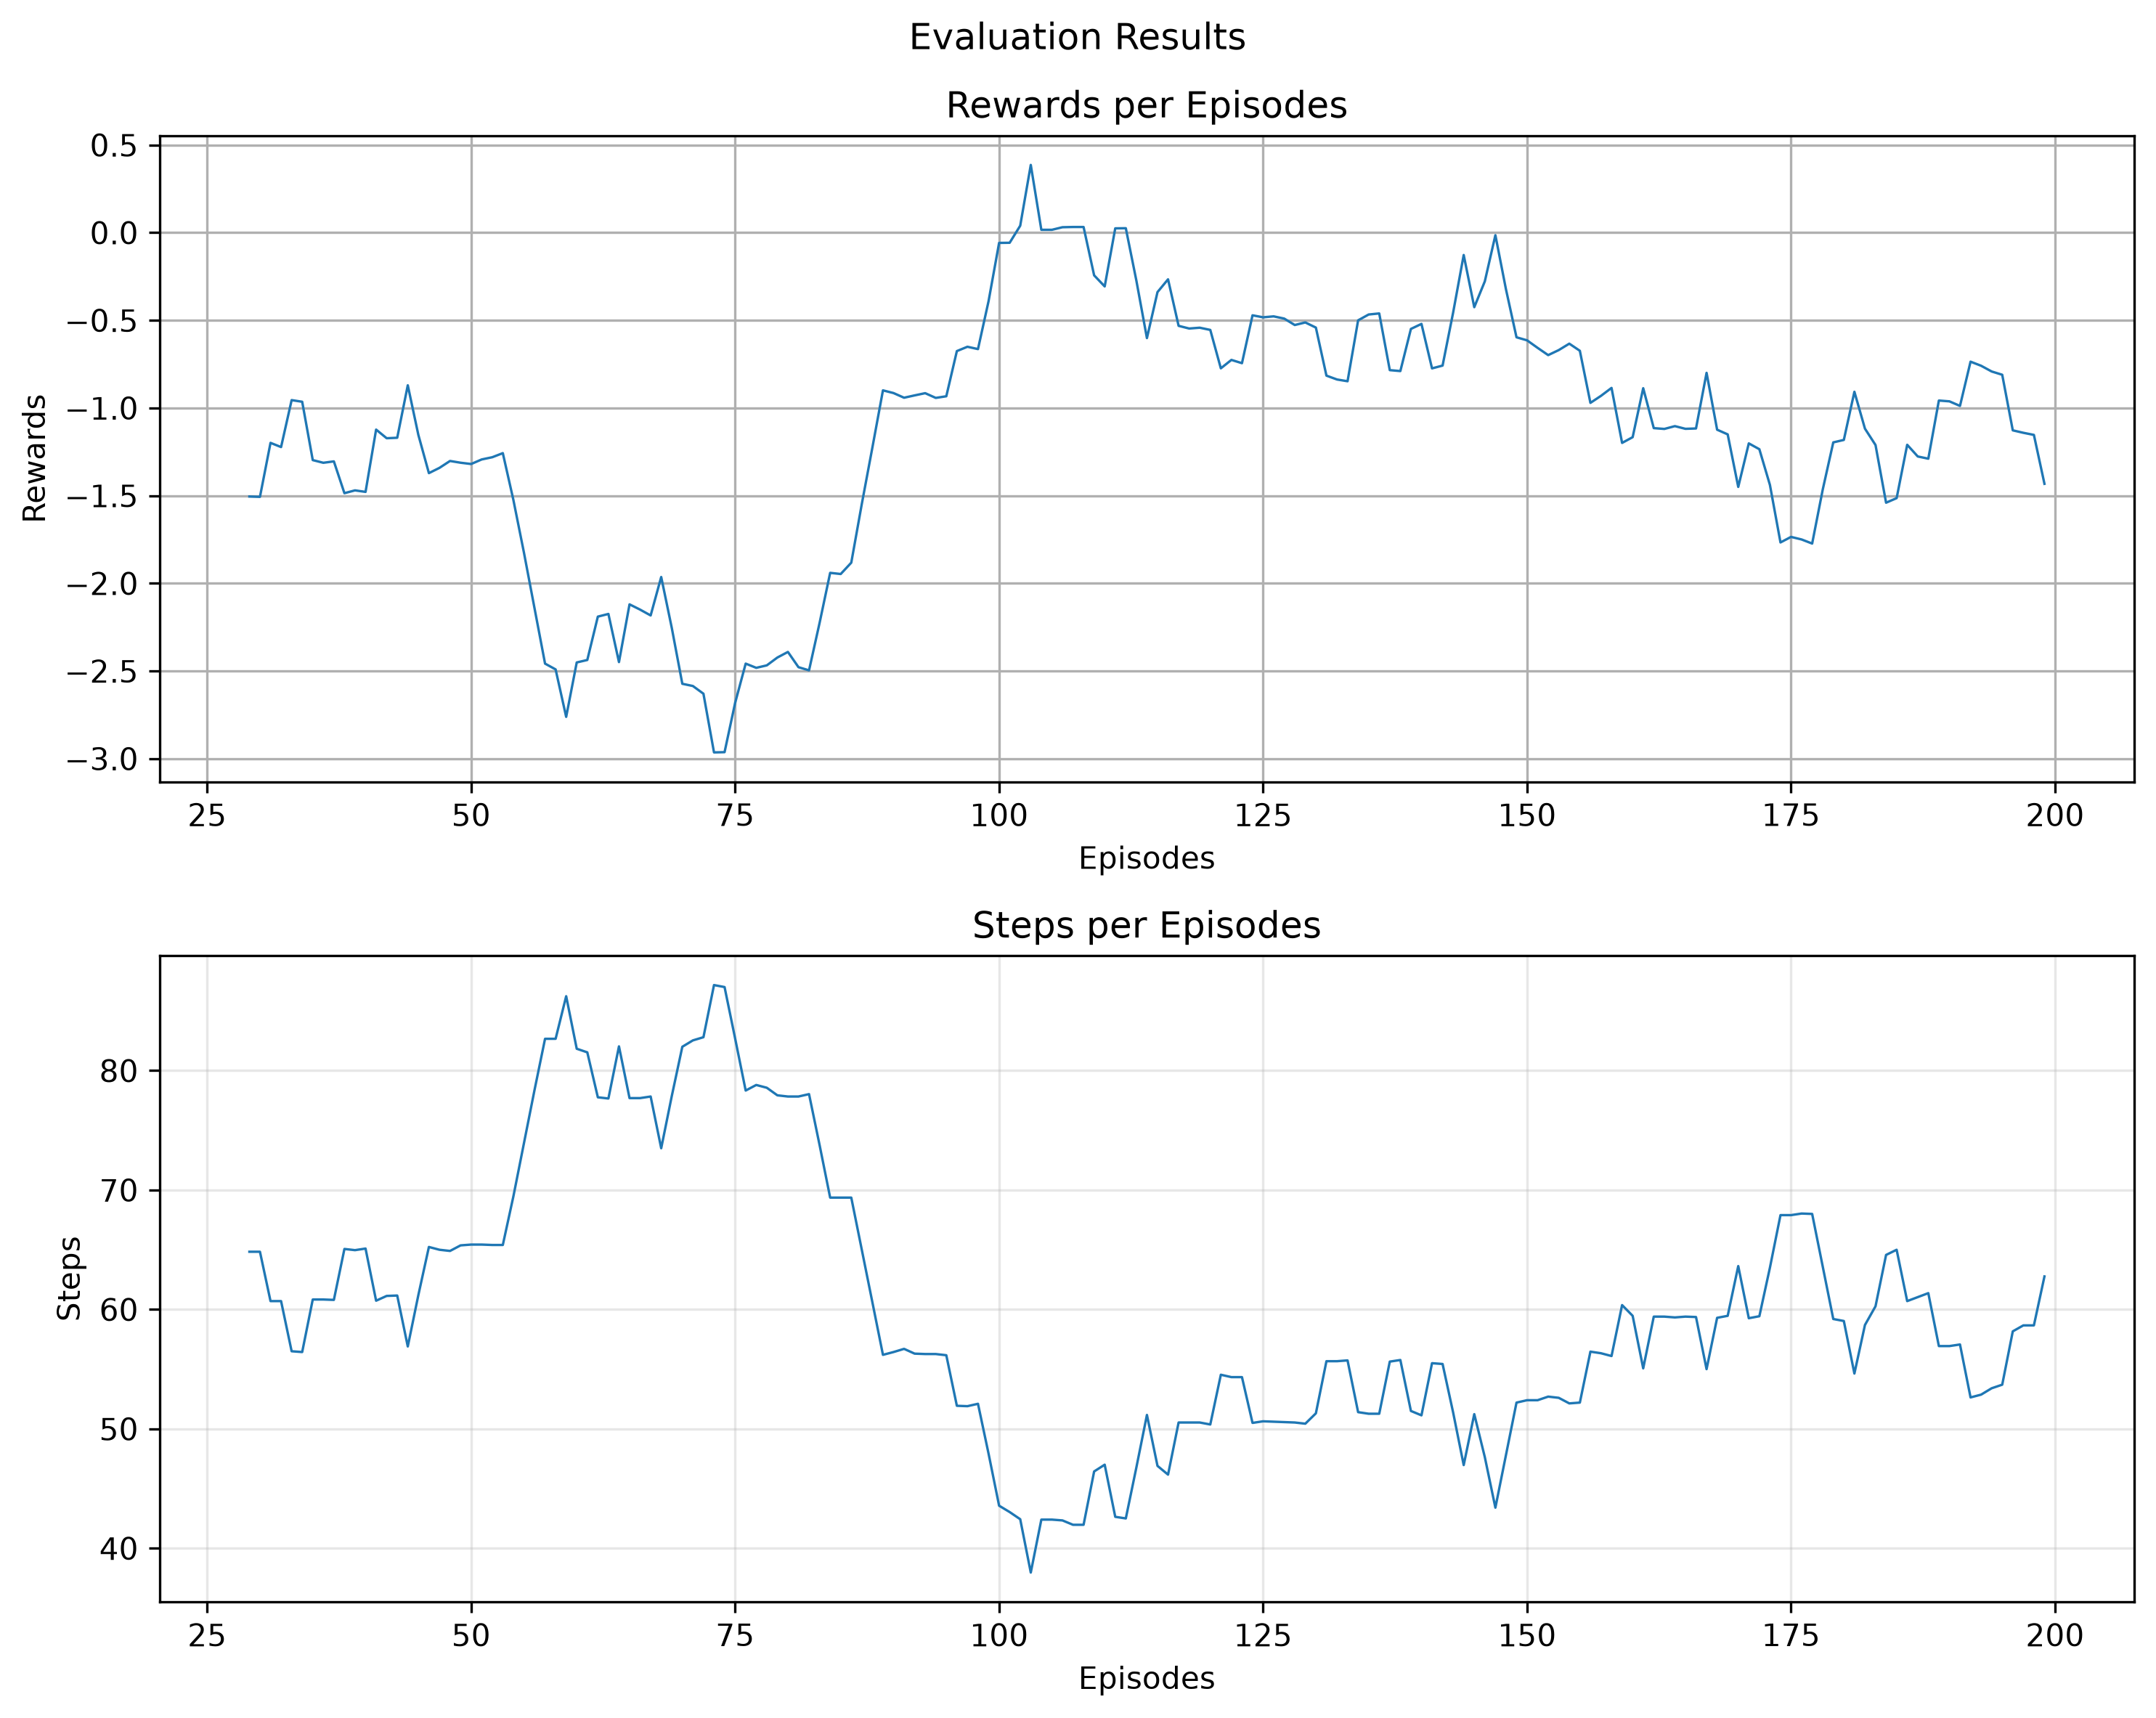
\includegraphics[width=0.72\textwidth]{./img/dqn_eval.png}
        \caption{DQN randomized-grid evaluation rewards and steps over 200 episodes. Higher rewards and fewer steps indicate successful, efficient routes.}
        \label{fig:dqn-evaluation}
    \end{figure}

    Figure~\ref{fig:dqn-training} shows that DQN learning is not immediate: early episodes routinely end at the 150-step limit with strongly negative rewards.
    The moving averages then improve substantially before oscillating, indicating that the 3,000-episode run learned useful motion but remained sensitive to map layout and stochastic failures.
    Figure~\ref{fig:dqn-evaluation} shows the same tradeoff during evaluation: successful episodes usually require fewer than 30 steps, while unsuccessful episodes consume the full limit.

    \begin{table}[htbp]
        \centering
        \begin{tabular}{lcc}
            \hline
            \textbf{Method} & \textbf{Successful / Episodes} & \textbf{Success Rate} \\
            \hline
            Random policy & 75/1,000 & 7.5\% \\
            DQN (systematic evaluation) & 140/200 & 70.0\% \\
            DQN (rendered test) & 4/5 & 80.0\% \\
            Q-learning (rendered test) & 9/10 & 90.0\% \\
            \hline
        \end{tabular}
        \caption{Final baseline and policy comparison. The two rendered-test runs use different sample sizes, so success rates should be interpreted alongside the larger systematic evaluations.}
        \label{tab:test-results-comparison}
    \end{table}

    \begin{figure}[ht]
        \centering
        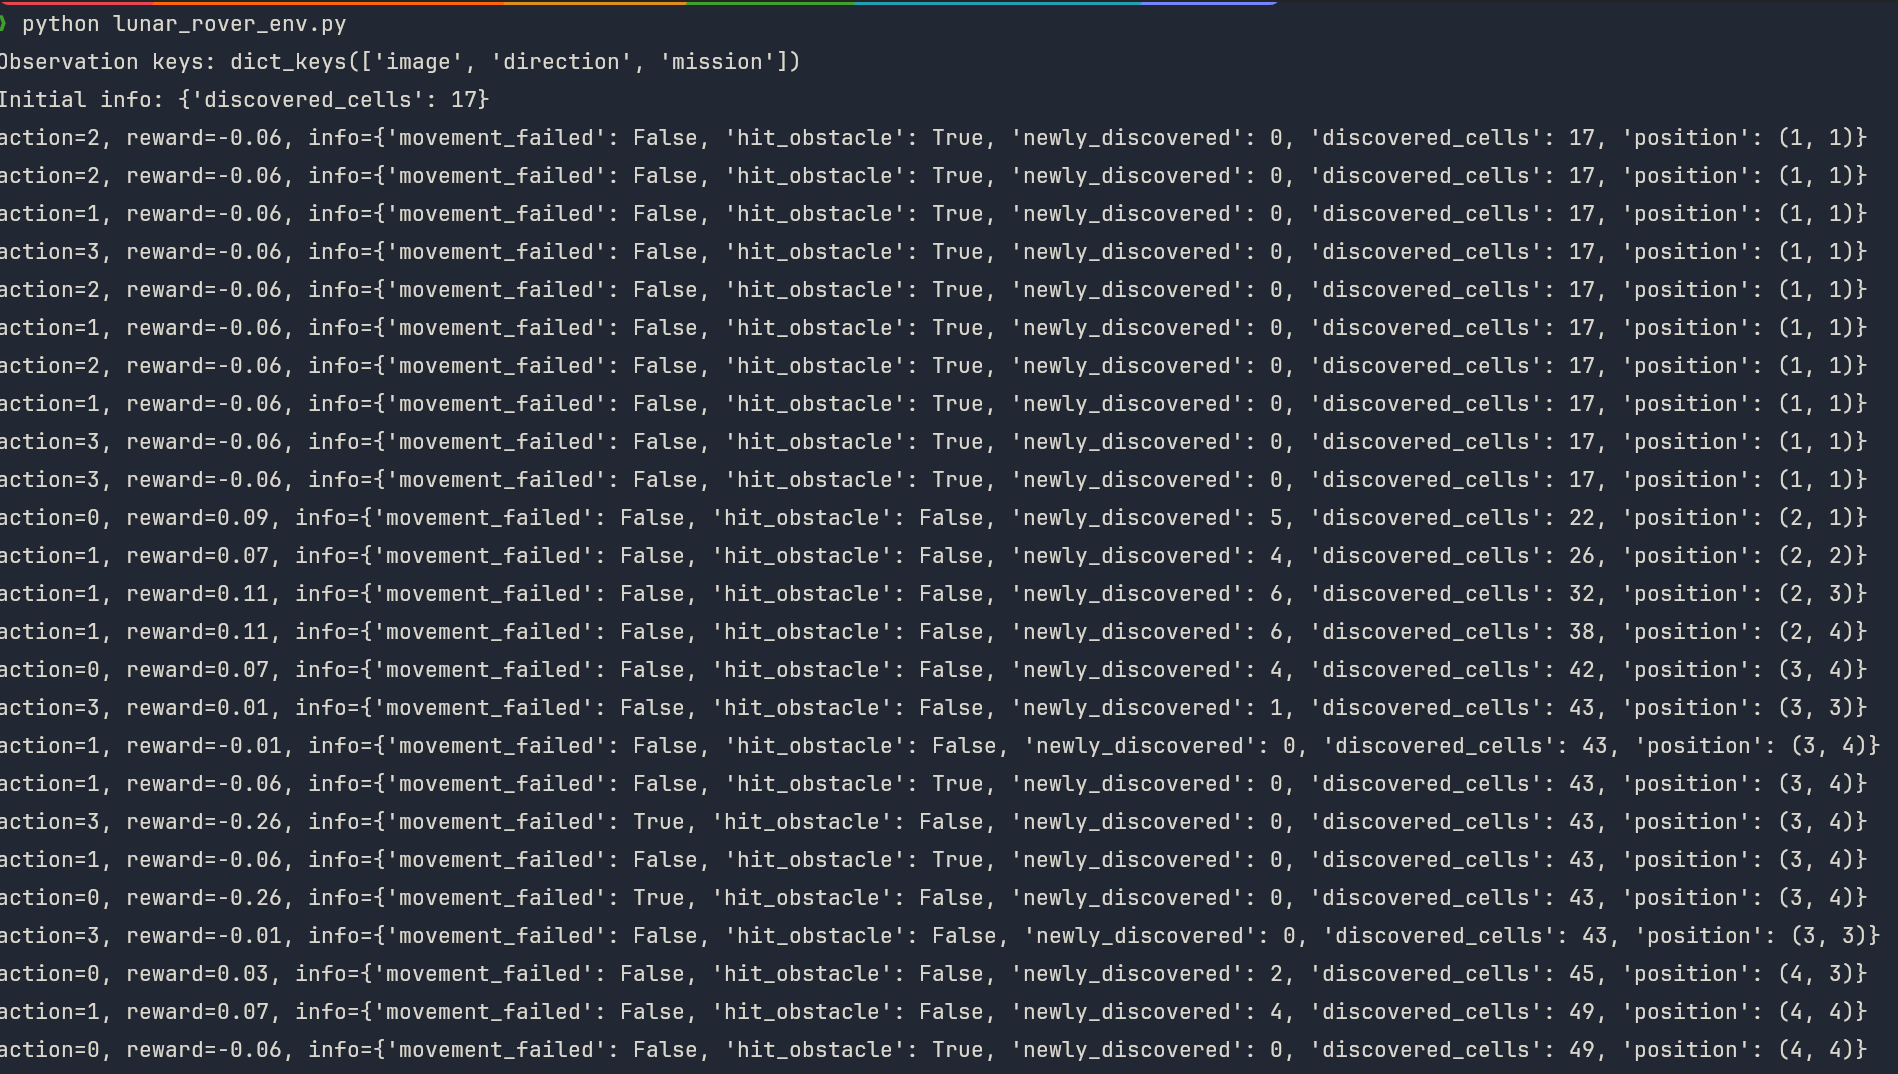
\includegraphics[width=0.72\textwidth]{./img/test_run_output.png}
        \caption{Rendered test output from the final demonstration. It records episode outcomes, average reward, and average steps.}
        \label{fig:test-output}
    \end{figure}

    Table~\ref{tab:test-results-comparison} shows that both learned approaches exceed the random baseline.
    In the large DQN evaluation, average reward was $-1.233$ and average episode length was 61.175 steps.
    The rendered DQN test completed 4 of 5 episodes successfully, averaging $-0.178$ reward and 45.2 steps.
    The rendered randomized-grid Q-learning test completed 9 of 10 episodes, averaging $0.218$ reward and 41.7 steps.
    These small rendered samples are not a claim that Q-learning dominates DQN; they demonstrate that the tabular policy can still achieve strong point estimates on the specific test grids, whereas DQN is better supported by the 200-episode generalization run.
    A direct difference in test sample size also prevents the 80\% and 90\% rendered results from being treated as statistically definitive.

    %-----------------------------------------%
    \section*{Discussion \& Limitations}
    Replay memory and target-network updates allowed DQN to improve over a policy that initially failed nearly every episode.
    However, training rewards and success rates remain uneven, and the 70\% systematic evaluation still falls below the project's 80--90\% target.
    The first major limitation is partial observability: the rover does not receive global obstacle coordinates, so a learned policy must infer routes from short local views.
    The second is stochastic movement, where a valid action sometimes fails and causes the episode path to diverge from the training batch.
    The final 200-episode DQN run reached 70\% success, while the 5-episode rendered test reached 80\%; this variation is expected for a relatively small test set on random maps.

    Q-learning's favorable 90\% rendered result should not be interpreted as equivalent generalization to DQN's 70\% systematic result.
    The 200-episode tabular-evaluation CSV used for the current project contains 100\% success and a 24-step fixed result in the reported configuration, but that evidence is too sensitive to the selected grid and seed.
    It does show that Q-learning can solve repeated or favorable layouts, consistent with earlier work; DQN was selected because replay and nonlinear function approximation provide a more credible approach to varying layouts.
    Future work should use the same fixed set of seeds and an equal number of episodes for every method, report confidence intervals, tune exploration and reward shaping, and compare additional DQN architectures.
    Longer DQN training alone is unlikely to solve partial observability; adding a recurrent or map-memory component would be a more meaningful robustness improvement.

    %-----------------------------------------%
    \section*{Conclusion}
    This project produced a complete random-grid lunar-rover environment and implemented, trained, and tested both tabular Q-learning and a DQN.
    The DQN improved moving-average training rewards and steps, reached 70\% success across 200 newly generated evaluation grids, and outperformed the 7.5\% random-policy baseline.
    It did not consistently achieve the intended 80--90\% success target.
    The main lesson is that replay and nonlinear function approximation improve the learned behavior, but partial observability, stochastic transition failures, and limited independent test runs continue to constrain reliable generalization.
    Future improvements should prioritize equalized multi-seed experiments and explicit memory of explored terrain, rather than changing only the final network size.

    \section*{Video Demonstration}
    Video 1: \texttt{test\_run.mp4}. The recording is under 60 seconds and demonstrates the rendered rover interacting with newly generated environments while summarizing the final test performance.

\end{document}
